\documentclass[num-refs]{wiley-article}
%\documentclass[blind,alpha-refs]{wiley-article}

\usepackage{amsmath,graphicx}
\usepackage{anyfontsize}
\usepackage{siunitx}
\usepackage{silence}


% Update article type if known
\papertype{Original Article}
% Include section in journal if known, otherwise delete
\paperfield{Journal Section}

\title{ Segmentation of prostate and prostate zones using Deep Learning: multiple MRI vendor analysis }
%\title{ Towards a universal MRI atlas of the prostate and prostate zones. Part II: Deep Learning }

% List abbreviations here, if any. Please note that it is preferred that abbreviations be defined at the first instance they appear in the text, rather than creating an abbreviations list.
\abbrevs{PZ, pheriperal zone; CNN, Convolutional Neural Network.}

% Include full author names and degrees, when required by the journal.
% Use the \authfn to add symbols for additional footnotes and present addresses, if any. Usually start with 1 for notes about author contributions; then continuing with 2 etc if any author has a different present address.
\author[1]{Olmo Zavala-Romero PhD}
\author[1]{Adrian L. Breto }
\author[1]{Nicole Gautney}
\author[1]{Yu-Cherng C. Chan}
\author[1]{Alan Dal Pra}
\author[1]{Alan Pollack}
\author[1]{Radka Stoyanova}
%\author[2]{Author B.~Four}

\affil[1]{Radiation Oncology, University of Miami Miller School of Medicine,
                Miami, FL, 33136, USA}

\corraddress{Olmo Zavala-Romero PhD, 
            Radiation Oncology, University of Miami Miller School of Medicine,
            Miami, FL, 33136, USA}

\corremail{osz1@med.miami.edu}

\fundinginfo{Funder One, Funder One Department, Grant/Award Number: 123456, 123457 and 123458; 
Funder Two, Funder Two Department, Grant/Award Number: 123459}

% Include the name of the author that should appear in the running header
\runningauthor{Olmo Zavala-Romero et al.}

\begin{document}
\maketitle

\begin{abstract}
A modified version of the 3D U-net  neural network architecture is used for automatic segmentation of the prostate and its peripheral zone (PZ) using multiplanar MRI. The network architecture is a multi-stream convolutional neural network (CNN) that uses axial, coronal, and sagittal MRI series as input.  A large dataset of 557 scans from multiple MRI vendors is used to analyze the consequences of training the CNN with distinct MRI magnets. The proposed segmentation scheme achieved good results for prostate and PZ compared to expert contoured volumes. Combining images from different MRI vendors on the training of the network is of paramount importance for training an universal model for prostate and peripheral zone segmentation. 

\keywords{ Prostate Cancer, Multi-parametric MRI, Deep Learning, U-Net, Machine Learning, Prostate Zones}
\end{abstract}

% 5000 words, 10 Figures and tables
\section{Introduction}
\label{sec:intro}
Accurate prostate segmentation on MRI datasets is required for many clinical and research 
applications. Furthermore, due to the different imaging properties of the peripheral (PZ) 
and transition zones (TZ) of the prostate, accurate zonal segmentation is also necessary. 
The prostate and zonal contours are necessary for computer aided diagnosis (CAD)
applications for diagnosis, staging, and treatment planning for prostate cancer. In 
series of applications, the prostate contours are fused with the ultrasound volume for 
to guide prostate biopsies. Automatic segmentation of the prostate, PZ and TZ on MR 
images provides an opportunity to broaden the current scope of research by facilitating 
studies that include large populations of subjects and/or studies that incorporate 
serial imaging of the prostate to provide a longitudinal picture of disease 
progression and response.  
Prostate MRI image segmentation has been an area of intense research \cite{litjens2014evaluation}. Earlier, the 
applied approaches varied from model-based \cite{chowdhury2012concurrent,toth2012multifeature},
 to atlas-based segmentation
\cite{4_klein2008automatic,5_cheng2014atlas, 6_xie2014low, 7_tian2015fully, 8_korsager2015use, 9_chilali2016gland}.
 Our group also evaluated the performance of atlas-based approach for prostate and prostate zones 
segmentation using data from different MR vendors and acquisition parameters\cite{10_padgett2018towards}. The advent 
of deep learning techniques, such as convolutional neural networks (CNN) has led to great success 
in image classifiation\cite{11_krizhevsky2012imagenet,12_simonyan2011immediate}. Recently, 
a U-net architecture has been proposed\cite{13_ronneberger2015u} for medical imaging 
segmentation and has been applied to the prostate\cite{14_meyer2018automatic}.
Here we present a modification of U-net architecture for segmentation both 
the prostate and prostate zones. In continuation of our previous work for creating an 
universal segmentation tool, the network is evaluated for images from different MR vendors.  

\section{Methods}
\label{sec:methods}

\subsection{Dataset}
\label{subsec:dataset}

The data


\subsection{Preprocessing}
\label{subsec:prepro}
The proposed preprocessing steps for the MRIs consist of bias correction using the N4ITK algorithm \cite{n4itk}, followed by image normalization to an interval of [0,1],  image re-sampling to uniform resolution, automatic selection of a region of interest (ROI), and (contour) interpolation.  

The MRI series are re-sampled to a resolution of $0.5 \times 0.5 \times 0.5$ mm  using linear interpolation \cite{itk}. The ROI, containing the prostate gland, is automatically obtained from the intersection of the rectangular prisms of the three MRI planes \cite{anneke}. The resampled ROI are  are linearly interpolated to an isotropic volume with a resolution of $168^3$. Figure \ref{fig_1} shows an example of an axial T2-w MRI before and after preprocessing.
% fig:fig_1

Contour preprocessing included interpolation using optical flow.  The manual contours were carried out on the original T2-w MRI resolution and hence the necessity for interpolation. The proposed method estimates 2D contours in-between slices of the axial plane and computes them independently for every two consecutive slices. First, optical flow is obtained between the two contours of adjacent slices using the Farneback method \cite{optflow}. Then, intermediate contours are generated by linearly interpolating the position of their edges following the direction of the optical flow vector field. Figure \ref{fig:fig_2} shows an example of the optical flow obtained between two horizontal slices and the resulting interpolated 3D volume using this method. 
% fig:fig_2

\subsection{3D-CNN architecture}
The proposed CNN consist of a 3D multistream architecture that follows the analysis and synthesis path of the 3D U-Net \cite{cciccek20163d}. Our implementation follows the one proposed by Anneke et al. in 2018  \cite{anneke}. The input of each stream is the post-processed ROI with a resolution of $168^3$ for one of three MRI series (axial, sagittal, and coronal). During the analysis phase, a combination of two convolutional layers and one max pool layer is grouped and repeated three times. The second convolutional layer in each set doubles the number of channels.  In the synthesis phase, a similar set of two convolutional layers and one deconvolution is applied three times. we modified the original network by implementing batch normalization \cite{ioffe2015batch} after each deconvolution and Dropout of 20\% \cite{hinton2012improving}.\\
We also cut down on the number of filters from $192$ to $28$ in the largest convolutional layer (after the first concatenation) reducing the number of parameters from to 995k to 663k in this layer. These changes reduced the training time in half as well the generalization of the  model. Figure \ref{fig:fig_3} shows the utilized model, all convolutional layers use a filter size of $3 \times 3 \times 3$ and rectified linear unit (ReLu) as the activation function; with the exception of the last layer which uses a filter size of $1 \times 1 \times 1$ and Sigmoid as the activation function to match the resolution of the input MRI series.
%\begin{figure*}[h]
%    \centering
%    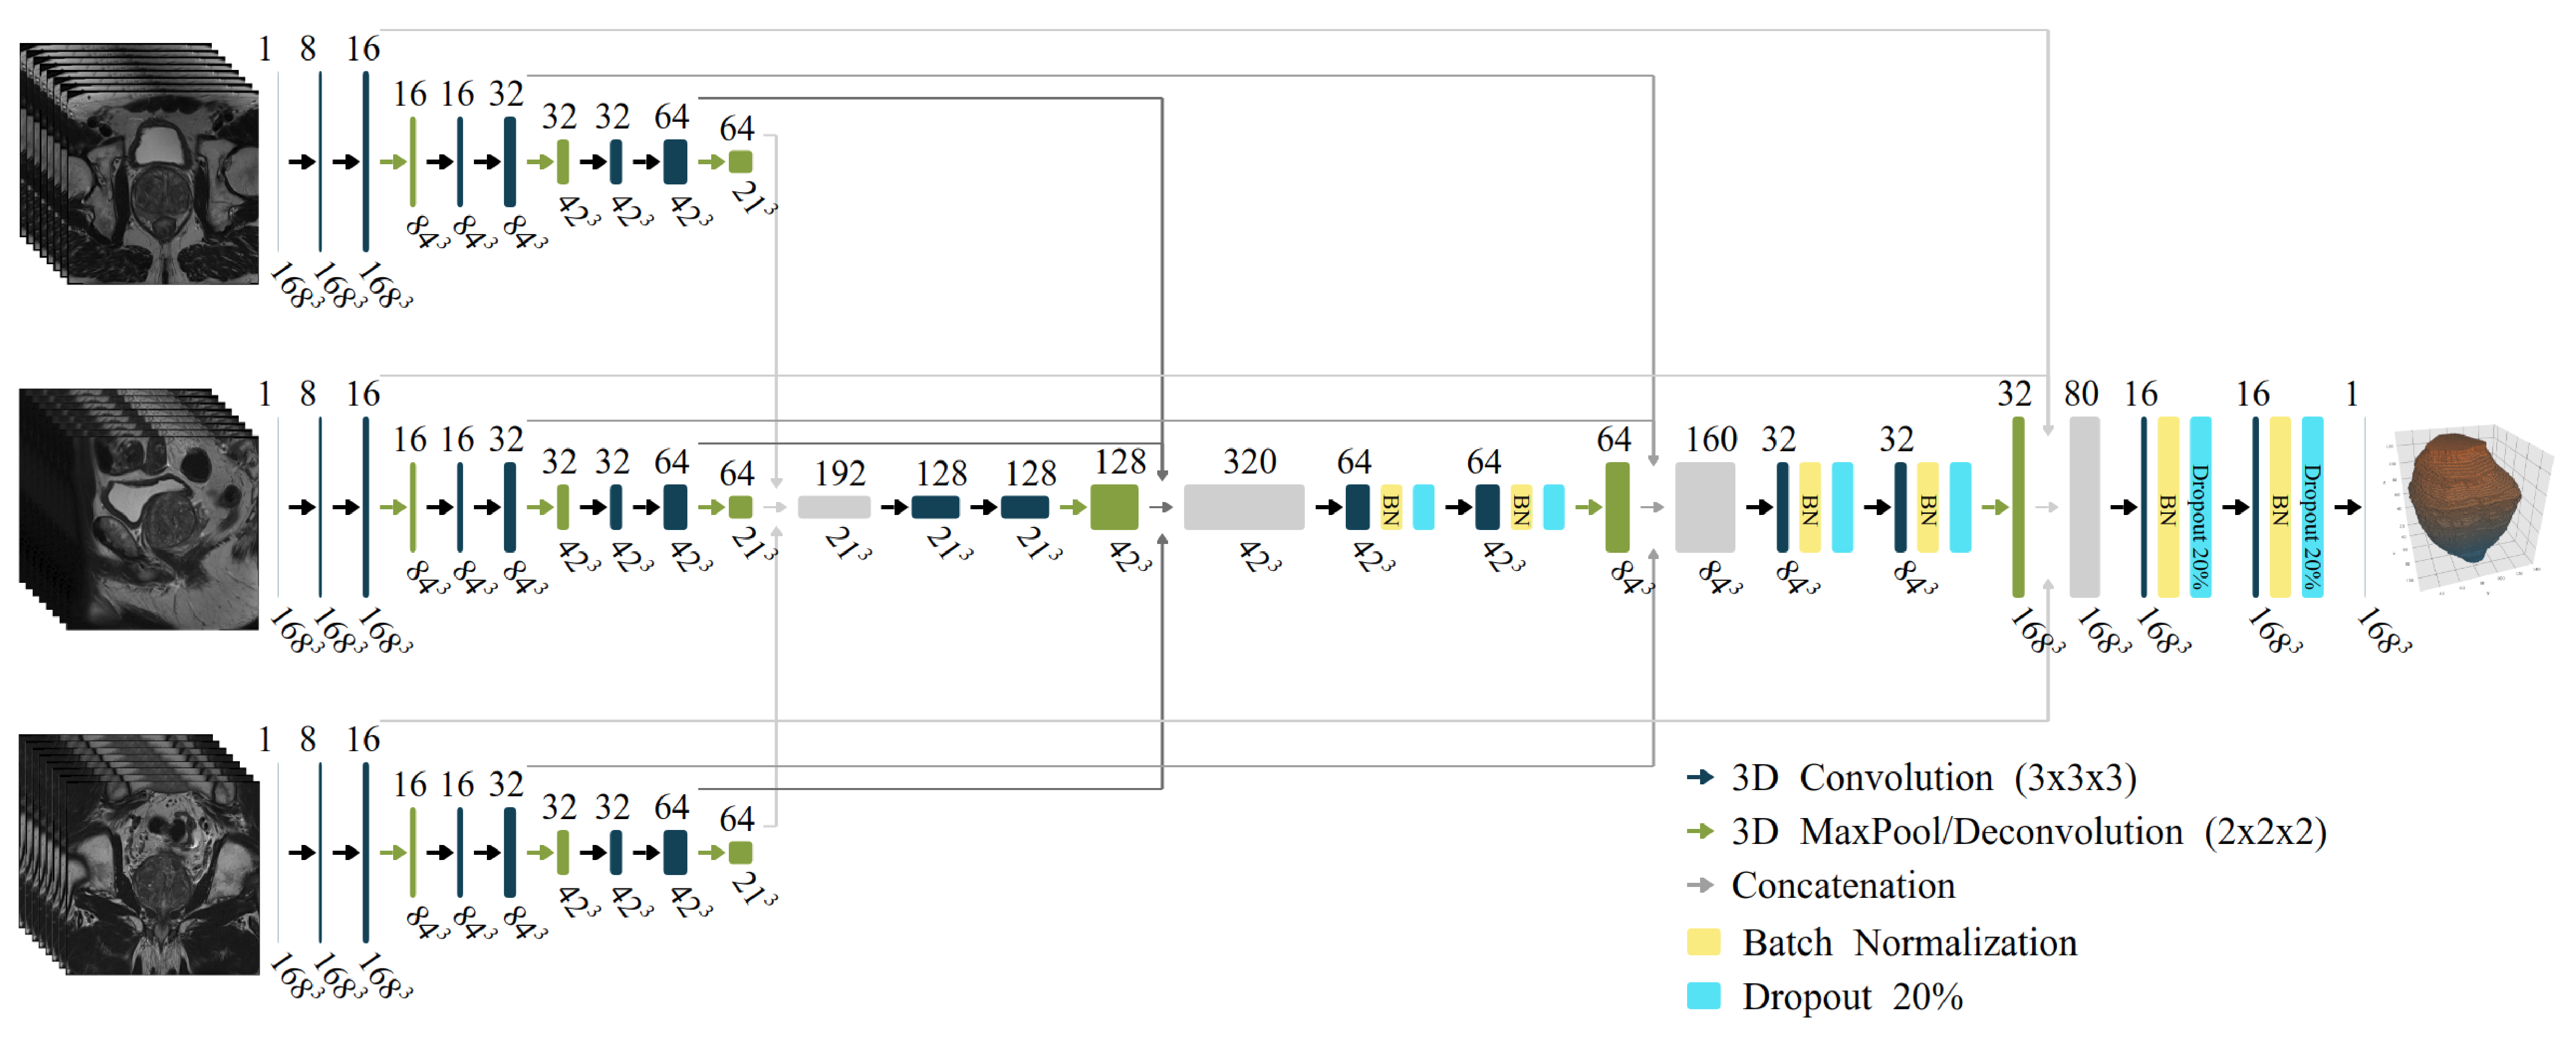
\includegraphics[totalheight=.282\textheight]{figures/Figure3.eps}
%    \caption{Multistream 3D convolutional network architecture. The input of the network are three $168^3$ volumes from the MRI planes: axial, sagittal, and coronal. }
%    \label{fig:fig_3}
%\end{figure*}
Finally, we demonstrate that even though the CNN was trained and tested on T2-w MRIs with sizes $168^3$, the final model is not restricted to that input size and could be used with different resolutions, as long as the field of view of the isotropic input volume being used is similar to the training data. 

\subsection{Training}
\label{subsec:training}
The selected optimization algorithm is Stochastic Gradient Descent (SGD) with a learning rate $\alpha = 0.01$, momentum of 0.9 and decay of $10^{-6}$. The training is performed for 1000 epochs with an early stop mechanism if the loss function is not improved by at least $\delta = 0.001$ after 70 iterations. 

The Loss function used for the training is the negative Dice Similarity Coefficient (DSC)(Dice, L. R. Measures of the Amount of Ecologic Association between Species. Ecology 26, 297-302, doi:Doi 10.2307/1932409 (1945)):  
\begin{equation}
\text{Loss} = - \frac{2 \sum_{i=1}^{N}p_it_i}{\sum_{i=1}^{N}p_i^2 + \sum_{i=1}^{N}t_i^2 + \varepsilon} 
\label{eq:dsc}
\end{equation}
%where N is the total number of voxels in the image, when training for prostate segmenation,
%and the number of voxels \textbf{inside} the prostate, when training for the PZ. The segmentation
%of the PZ assumes that we already know where the prostate is, so we do not take into
%account anything outside the prostate for the loss function. 
where N is the total number of voxels in the image, $p_i$ the voxel values for the prediction of the network, and $t_i$ the true voxel values of the prostate or PZ masks.

In order to compare the robustness of the models with respect to changes in MRI vendor machines,  a distinct model was trained for each dataset: GE (n=220), Siemens (n=330), combined model (n=550). Each dataset was split into 90\% for training and 10\% for validation. Data augmentation was performed on the fly by flipping the axail images in the sagittal axis and blurring them using 3D Gaussian blur up to $\sigma = 3$. Each data augmentation method is applied with a random chance of $1/2$.  
A total number of 6 models were trained from the combination of three datasets, and training for the segmentation of the prostate or the PZ. 

\subsection{Postprocessing}
The CNN outputs a 3D volume of the same size of the ROI, in our case $168^3$. From this cube, a binary mask is obtained by thresholding it with a value of 0.5. After that, we select the largest connected volume and remove all others. Finally, we compute the 3D DSC for the contour of interest in the resampled image and in the original MRI resolution. Additionally, the prediction of the PZ contour is intersected with the prostate, restricting it to the prostate volume.


\section{Results}
Table \ref{tab:res_prost} shows the obtained DSCs for the segmentation of the prostate when the three trained models are used for segmenting the GE and the Siemens dataset. The displayed DSCs are computed from the validation set when the model is trained on the same MRI vendor, and are calculated from the whole dataset when the model is trained from data of a different MRI vendor.

% tab:res_prost
When the model is trained with examples from one dataset and used to segment prostates from scans of the same MRI vendor the average DSCs are $0.855$ for GE and $0.892$ for Siemens. When the datasets are combined during training, the average DSC are $0.830$ for GE and $0.896$ for Siemens.  The results obtained for the Siemens dataset are comparable with recent methods for prostate segmentation \cite{guo2016deformable, lozoya2018assessing, jia20183d}. When the model is trained with examples from one MRI vendor and then used to process images from a different vendor, the resulting DSCs are lower ($0.262$ and $0.804$). We attribute this large discrepancy in DSCs for cross training and testing, to the difference in variability within the GE and Siemens dataset. The Siemens dataset is more homogeneous than the GE datasets, which makes its model less robust to changes but, at the same time, the Siemens model is better for segmenting images scanned from the same MRI machine. These results exhibits how sensible the model is for subtle changes in the training dataset and it also displays the importance of testing how well deep learning architectures in the medical field generalize to other MRI vendors. 

Figure \ref{fig:resseg} shows the middle axial slice for the lowest, closest to mean, and highest DSC obtained for prostate segmentation on the Siemens and GE dataset. In general, the DSC increases with respect to the volume size of the prostate, and predictions for the Siemens dataset follow better the contours from the experts. From these examples it is also clear the the images obtained with the Siemens machine have better native resolution than the ones from GE, which may be another reason why the network performs better for this MRI vendor. 
% fig:resseg

Table \ref{tab:res_pz} shows the obtained DSCs for the segmentation of the PZ for the three trained models.  The best DSCs of $0.797$ and $0.813$ are obtained when the model is trained using the combined dataset.  

% tab:res_pz
The average DSCs of all the PZ models are lower than the coefficients for segmenting the prostate, which implies that PZ segmentation is a more challenging task. The obtained DSC for segmenting the PZ with the \emph{Combined} model (0.788 and 0.811) are better than what we found in the literature for similar databases (0.60, 0.68, 0.62, 0.75) \cite{mooij_automatic_2018,toth_simultaneous_2013, chilali_gland_2016, hutchison_pattern_2012}. Figure \ref{fig:ressegpz} shows the middle axial slice for the lowest, closest to mean, and highest DSC obtained for the segmentation of the PZ on the Siemens and GE dataset. 
% fig:ressegpz 
\section{Discussion/Conclusions}
\label{sec:disc}
Manual contouring of the prostate requires slice-by-slice contouring in axial or in any of the other two views. Besides labor intensive, manual contouring is prone to inter-observer variability and imperfections in the 3D delineation. The 3D CNN results in this paper show that in addition to efficiency and reproducibility, automatic prostate and PZ segmentation can be achieved with accuracy, similar to the expert's manual contours results. Our robustness tests show a strong sensibility of this deep learning architecture with respect to the MRI vendor used for training. 



%\newpage
\textbf{Tables}
\begin{table}[ht]
    \caption{MRI acquisition parameters. The GE dataset was acquired in two modalities: large field of view (LFOV) and small field of view (SFOV). The Siemens dataset, was only acquired in the SFOV modality.}
    \begin{tabular}{lcccccc}
         \hline
          \textbf{Magnet} & \textbf{Plane} & \textbf{FOV} & \textbf{ET Min - Max} & \textbf{RT Min - Max} & \textbf{Matrix} & \textbf{Voxel size (mm)} \\
          GE & Axial & LFOV (n=100) & $81.31 - 105.50$ & $4806 - 10998$ & $256 \times 256 \times 72$ & $1.25 \times 1.25 \times 2.5$ \\
          GE & Axial & SFOV (n=120) & $80.88 - 93.48$ & $3700 -7078$ &
                \shortstack{ $256 \times 256 \times 27$ to\\ $512 \times 512 \times 37$} & 
                \shortstack{ $0.3906 \times 0.3906 \times 3$ to\\ $0.7813 \times 0.7813 \times 3$} \\
          GE & Coronal & SFOV (n=220) & $80.49 - 134.17$ & $1968 - 8006$ &  
                \shortstack{$320 \times 320 \times 32$ to \\  $512 \times 512 \times 30$} & 
                \shortstack{$0.3906 \times 0.3906 \times 3$ to \\ $0.6875 \times 0.6875 \times 3$}\\
          GE & Sagittal & LFOV (n=25) & $88.32 - 94.70$ & $9000$ & 
                \shortstack{$512 \times 512 \times 25$ to \\  $512 \times 512 \times 40$} & 
                $0.429688 \times 0.429688 \times 3$\\
          GE & Sagittal & SFOV (n=195) & $80.49 - 134.51$ & $2124 - 7917$&  
                \shortstack{ $256 \times 256 \times 25$ to \\ $512 \times 512 \times 33$} &
                \shortstack{$0.3906 \times 0.3906 \times 3$ to \\ $0.7813 \times 0.7813 \times 3$}\\
          Siemens & Axial & SFOV (n=330)  & $101 - 108$ & $4030 - 8624$&  
                \shortstack{$256  \times 256 \times 17$ to \\ $640 \times 640 \times 23$} & 
                \shortstack{$0.3906 \times 0.3906 \times 3$ to\\ $0.7813 \times 0.7813 \times 3$} \\
          Siemens & Coronal & SFOV (n=330) & $97 - 110$ & $3080 - 6620$&  
                \shortstack{$256  \times 256 \times 19$ to \\ $320 \times 320 \times 23$} & 
                \shortstack{$0.5625 \times 0.5625 \times 3$ to\\ $0.8001 \times 0.8001 \times 4$} \\
          Siemens & Sagittal & SFOV (n=330) & $101 - 110$ & $3810 - 6830$&  
                \shortstack{$320  \times 320 \times 17$ to \\ $448 \times 390 \times 13$} &
                \shortstack{$0.5625 \times 0.5625 \times 3$ to\\ $0.571 \times 0.571 \times 4$} \\
         \hline
    \end{tabular}
    \label{tab:dataset}
\end{table} 

\newpage
\begin{table}[ht]
    \caption{Dice Similarity Coefficients (DSC) (mean $\pm$ SD) for prostate, segmented with each of the three trained models (GE, Siemens, and Combined). The results are presented for data from GE and Siemens MRI vendors and the DSCs are calculated on the interpolated (0.5 x 0.5 x 0.5 mm) and original MRI resolution.}
    \begin{tabular}{lcc}
         \hline
          \textbf{Prostate Models} & \textbf{GE (Interpolated/Original Resolution)} & \textbf{Siemens (Interpolated/Original Resolution)}\\
         \hline
         GE & $0.855\pm0.064$/$\mathbf{0.860\pm0.054}$ & $0.804\pm0.099$/$0.802\pm0.106$ \\
         \hline
         Siemens & $0.262\pm0.118$/$0.288\pm0.139$ & $0.892\pm0.038$/$0.889\pm0.035$ \\
         \hline
         Combined & $0.830\pm0.112$/$0.827\pm0.109$ & $\mathbf{0.896\pm0.037}$/$0.892\pm0.036$\\
         \hline
    \end{tabular}
    \label{tab:res_prost}
\end{table} 

\newpage
\begin{table}[ht]
     \caption{Dice Similarity Coefficients (DSC) (mean $\pm$ SD) for PZ, segmented with each of the three trained models (GE, Siemens, and Combined). The results are presented for data from GE and Siemens MRI vendors and the DSCs are calculated on the interpolated (0.5 x 0.5 x 0.5 mm) and original MRI resolution.}
    \begin{tabular}{lcc}
         \hline
            \textbf{PZ Models} & \textbf{GE (Interpolated/Original Resolution)} & \textbf{Siemens (Interpolated/Original Resolution)}\\
         \hline
         GE  & $0.767\pm0.093$/$0.759\pm0.089$ & $0.537\pm0.204$/$0.539\pm0.204$ \\
         \hline
         Siemens  & $0.591\pm0.223$/$0.591\pm0.219$ & $0.808\pm0.085$/$0.808\pm0.087$ \\
         \hline
         Combined & $\mathbf{0.797\pm0.093}$/$0.788\pm0.093$ & $\mathbf{0.813\pm0.079}$/$0.811\pm0.79$\\
         \hline
    \end{tabular}
    \label{tab:res_pz}
\end{table}

\newpage
\textbf{Figure legends:}
\begin{figure}[ht]
    \centering
    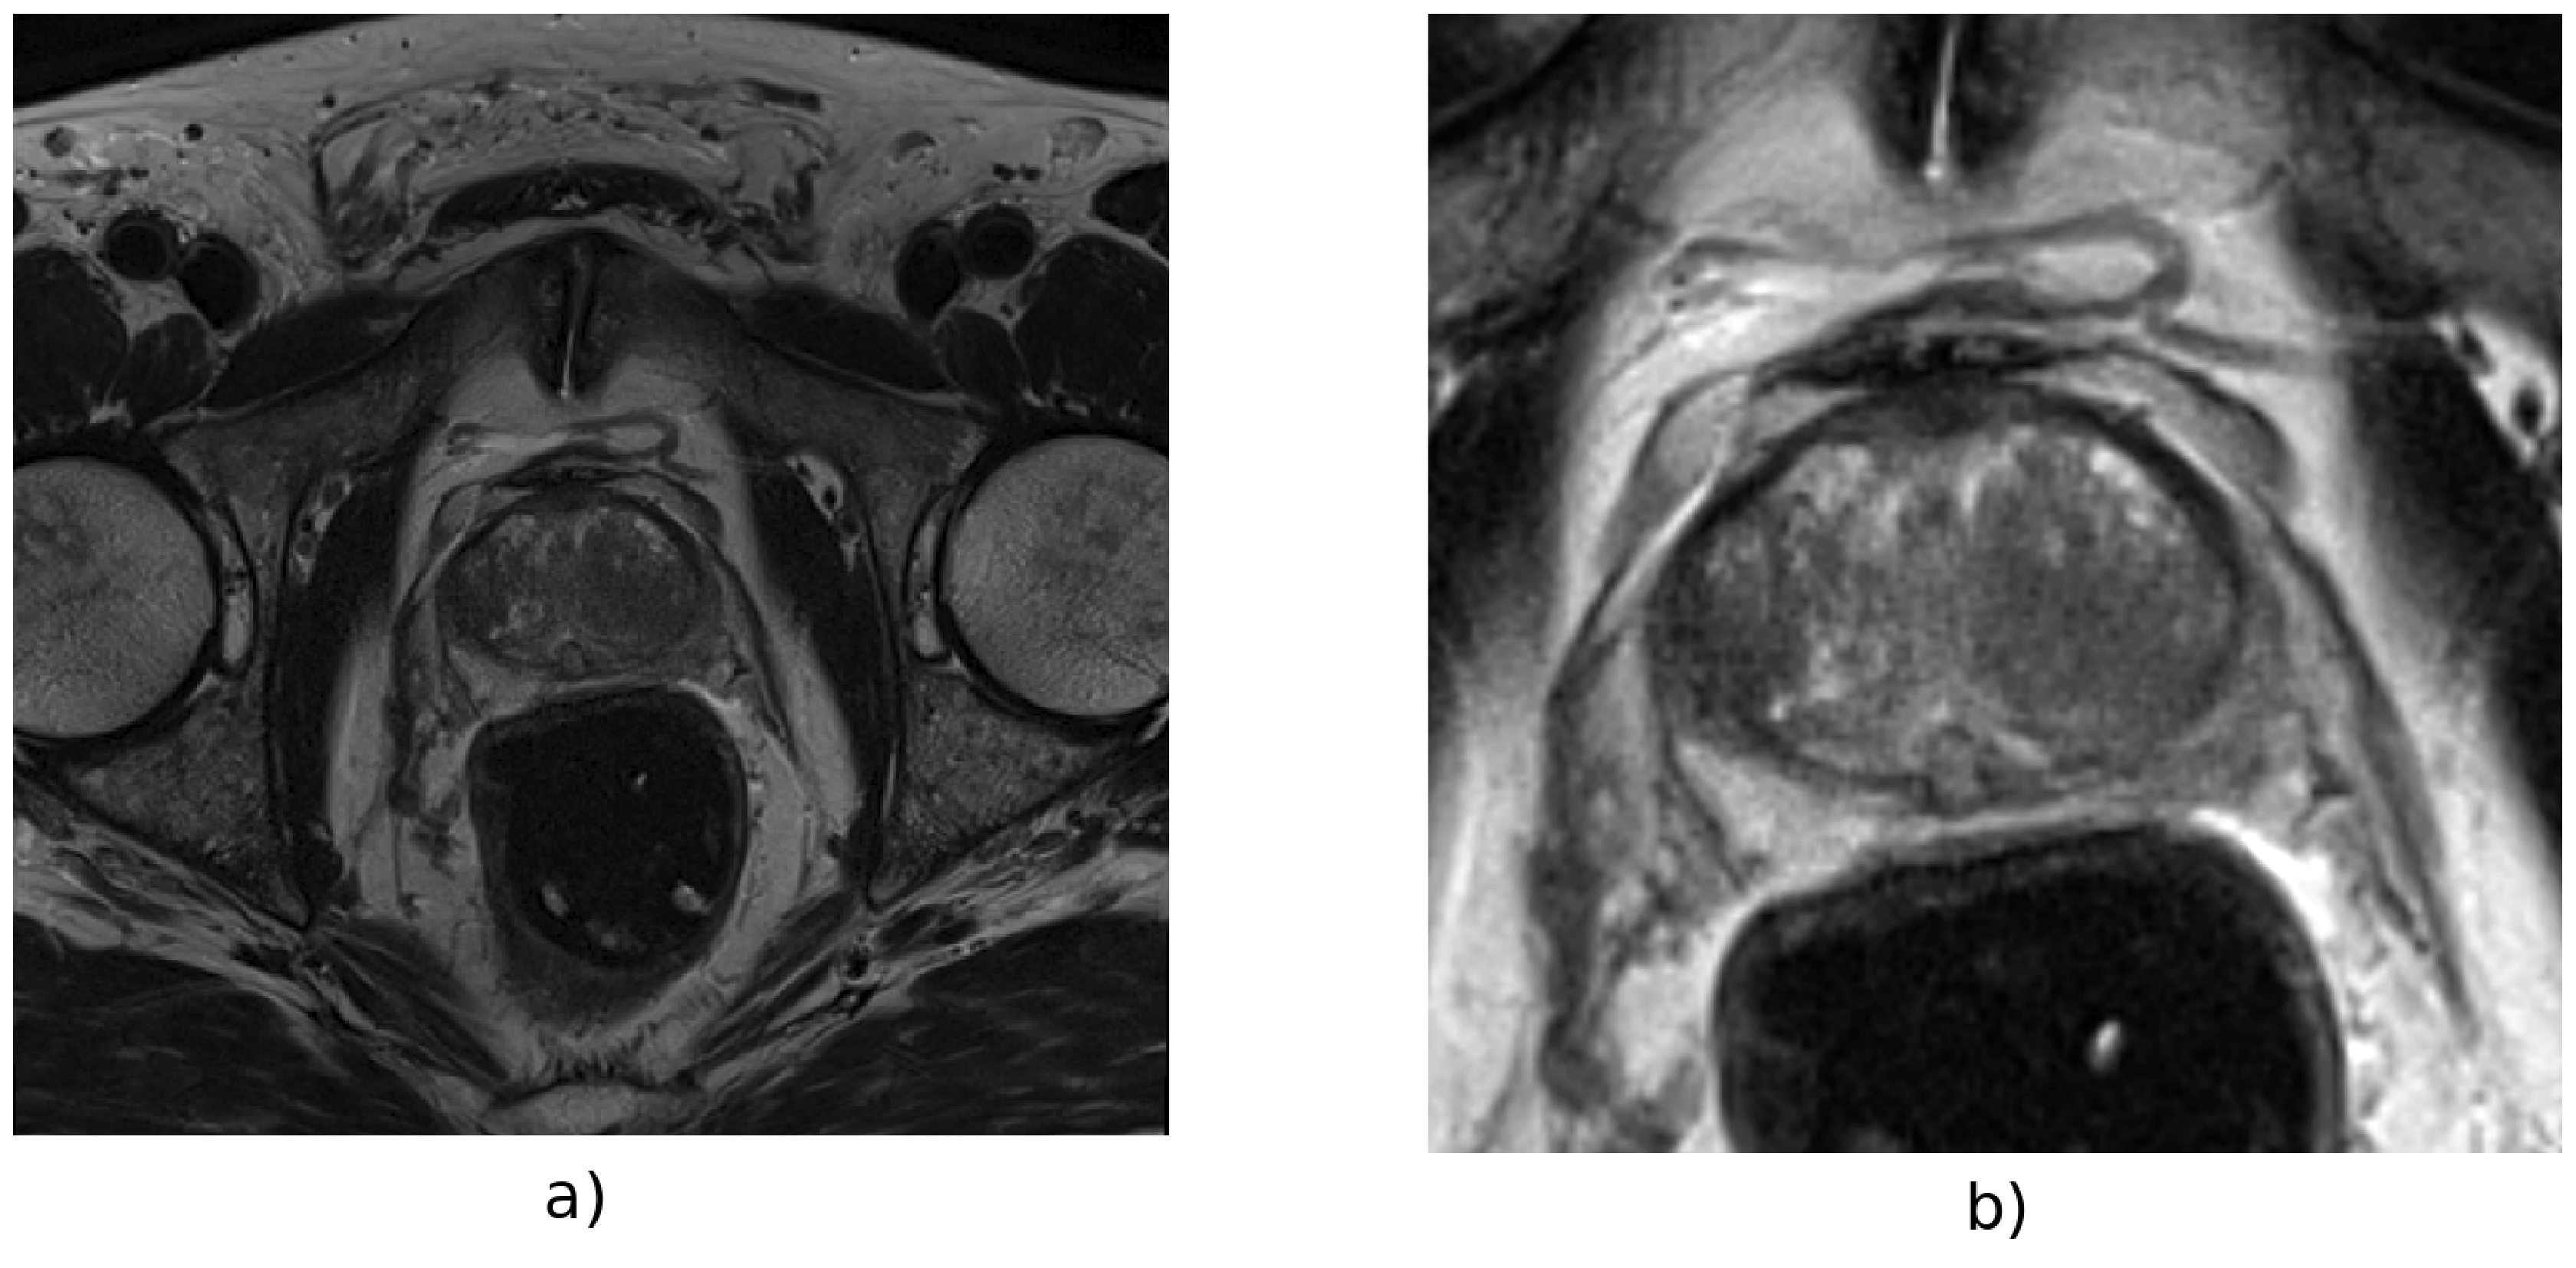
\includegraphics[totalheight=.25\textheight]{figures/Figure1.eps}
    \caption{Axial T2-weighted image \textbf{a)} before, and \textbf{b)} after preprocessing. Preprocessing steps include bias correction, intensity normalization, resampling, and cropping.} 
    \label{fig_1}
\end{figure}

\begin{figure}[ht]
    \centering
    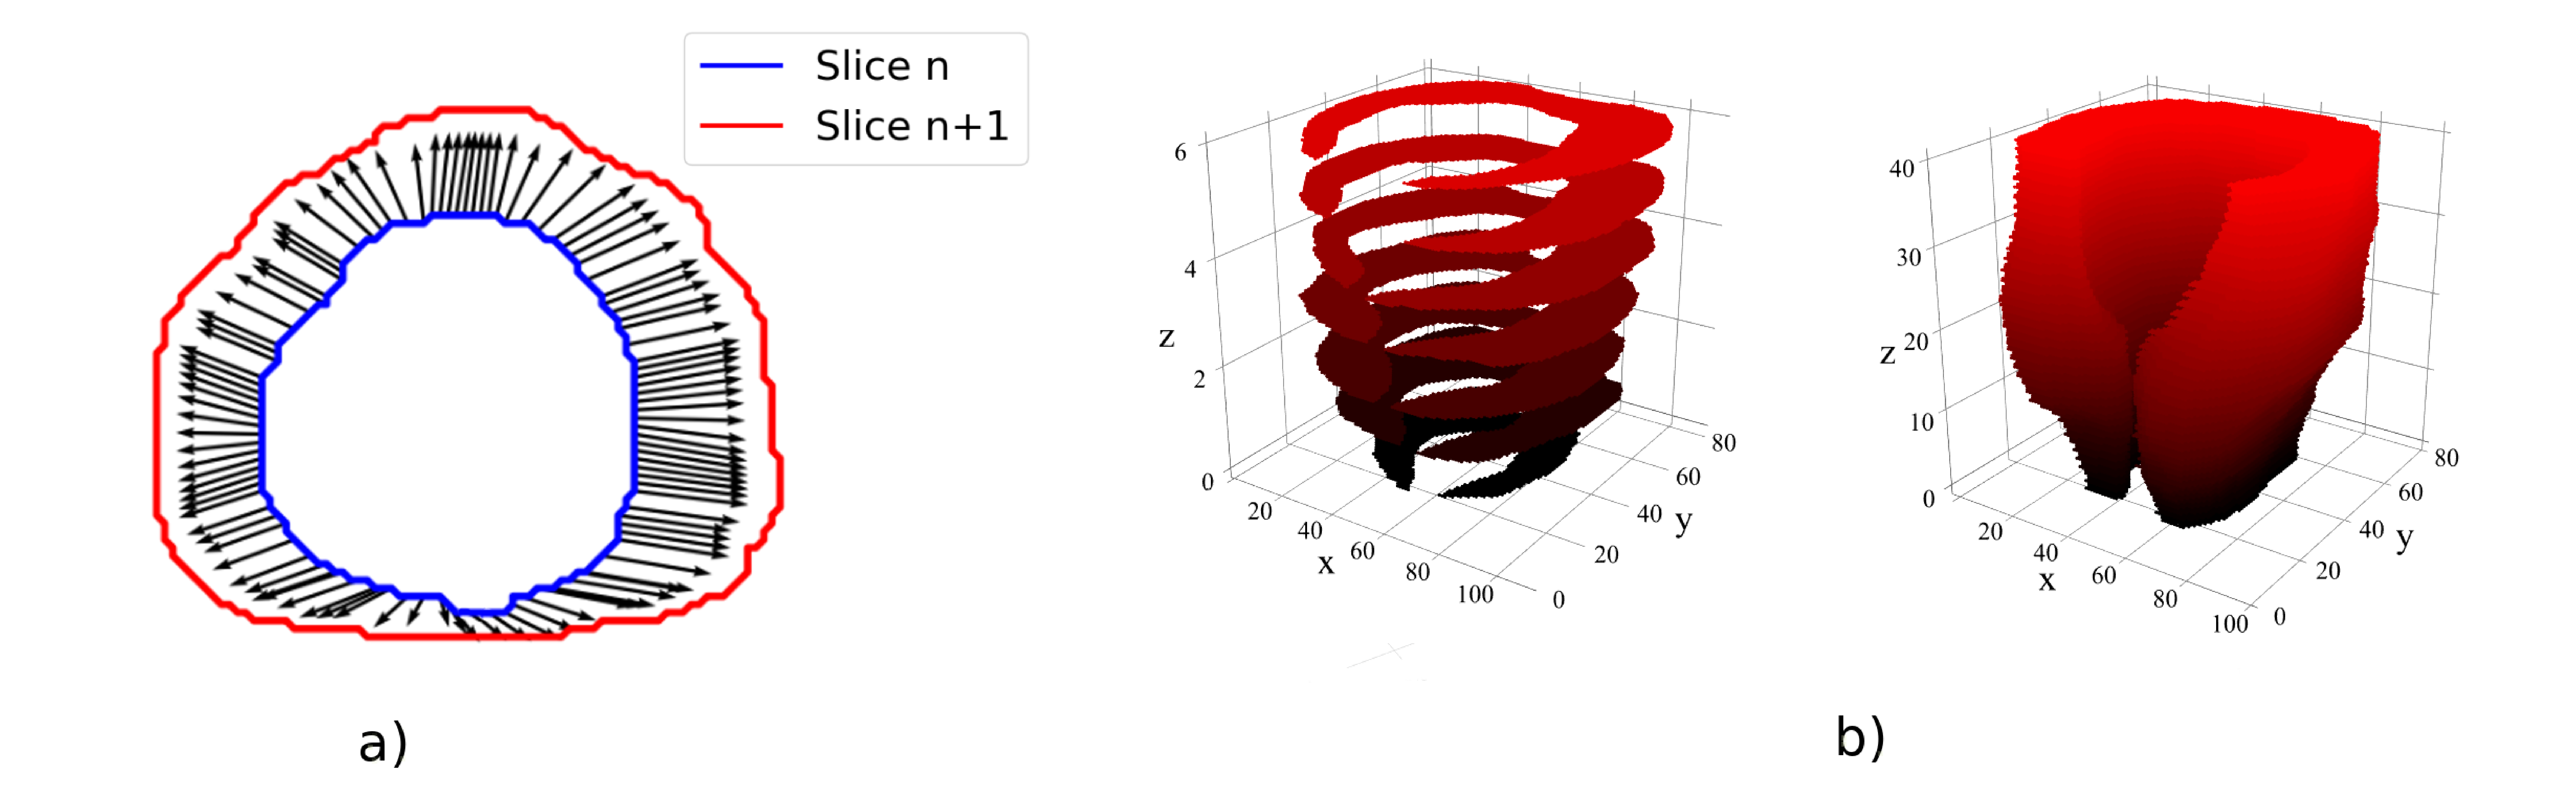
\includegraphics[totalheight=.21\textheight]{figures/Figure2.eps}
    \caption{Interpolation of prostate and PZ contours. \textbf{a)} an example of the optical flow obtained between two prostate contours from adjacent horizontal planes. In \textbf{b)} on the left, original contours with 17 slices. On the right, interpolated contours with 68 slices.}
    \label{fig:fig_2}
\end{figure}

\begin{figure*}[ht]
    \centering
    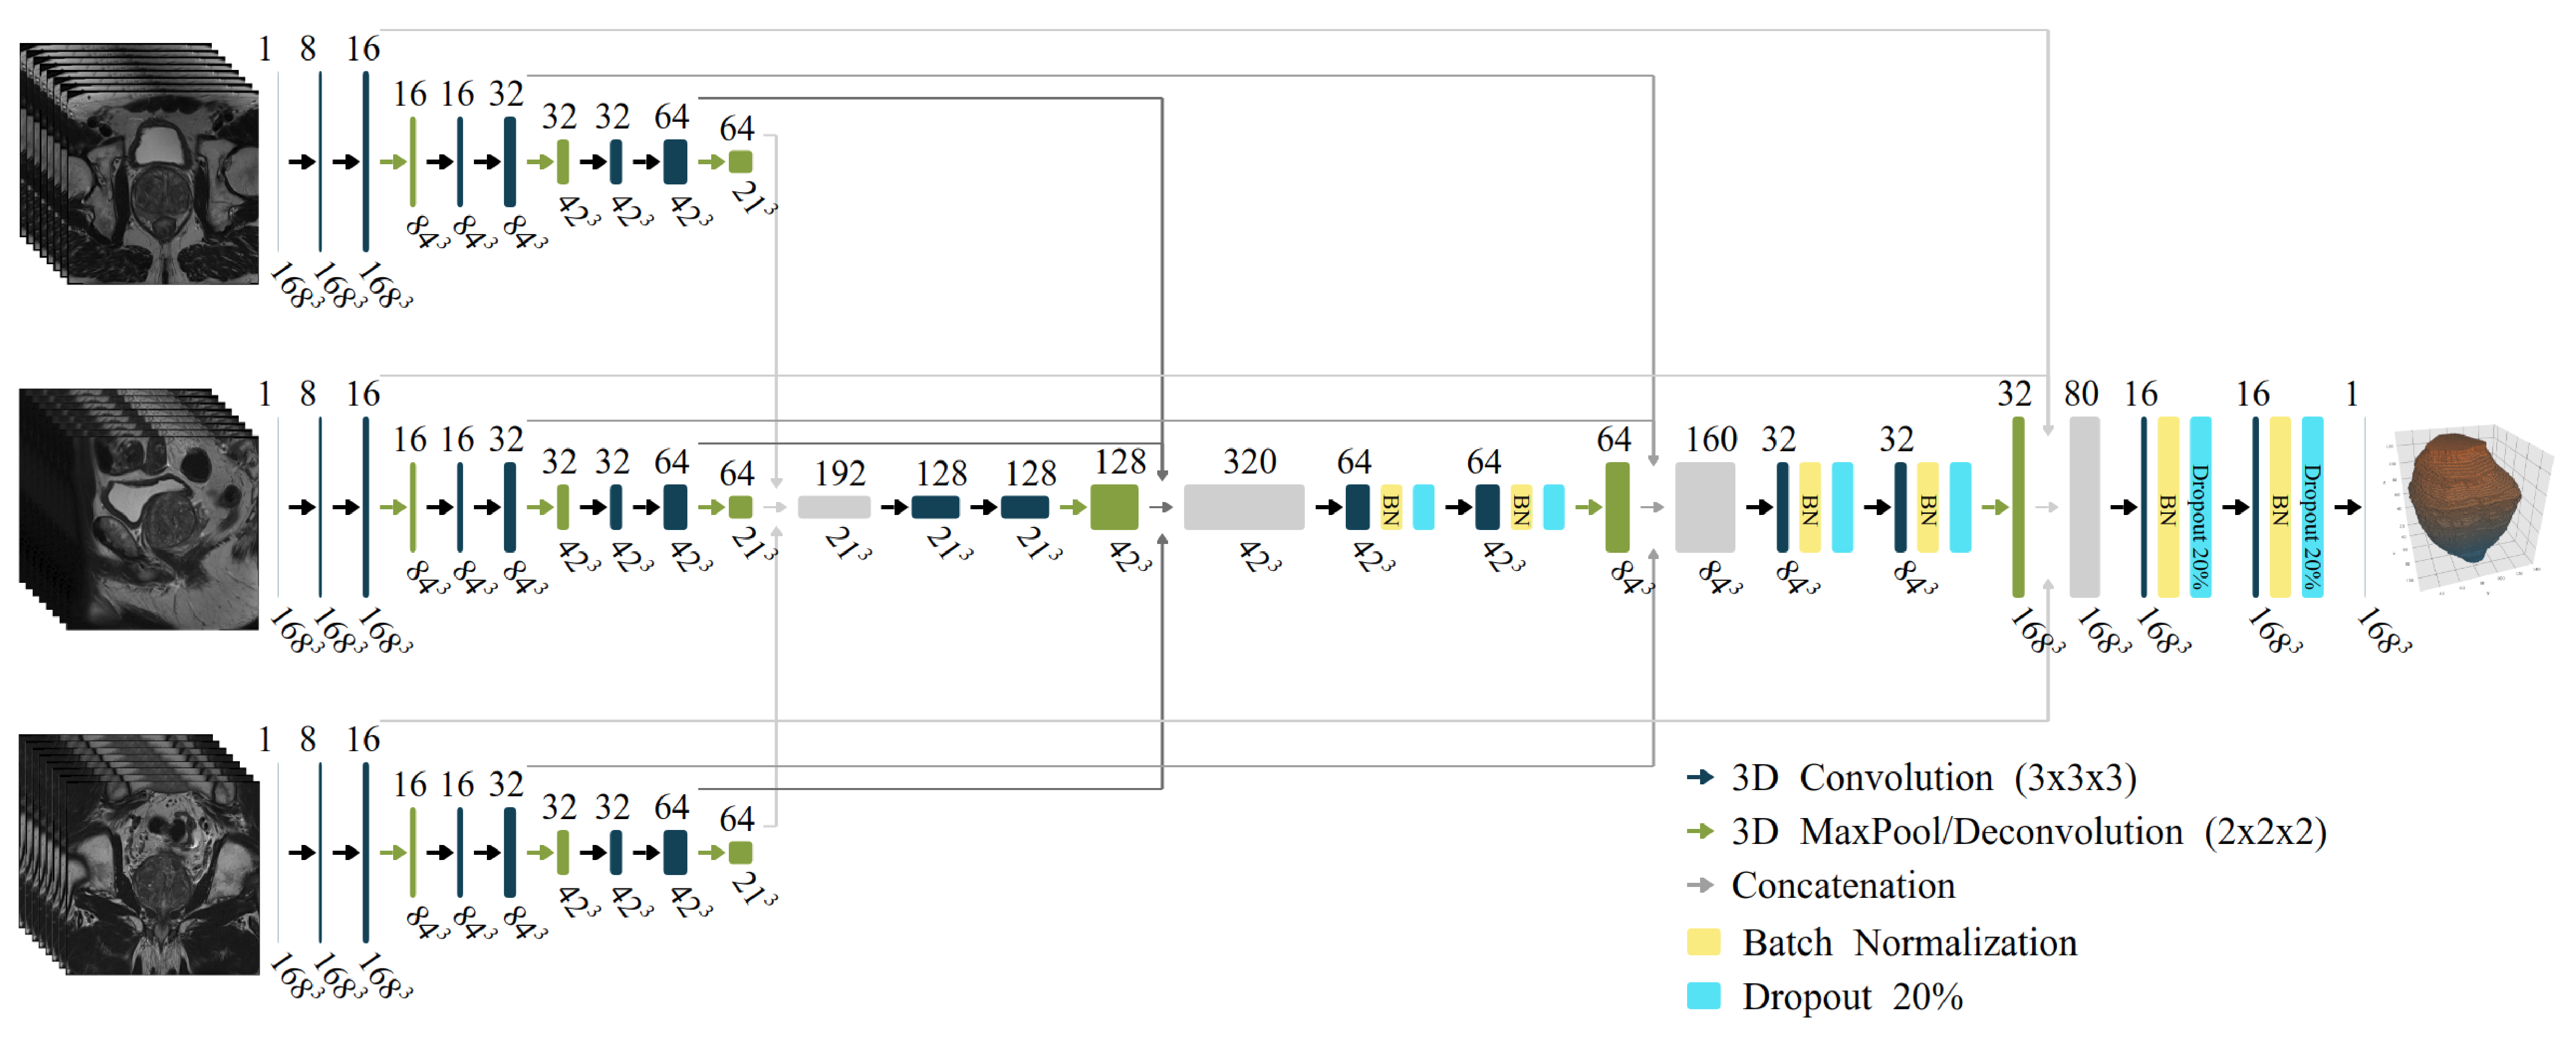
\includegraphics[totalheight=.282\textheight]{figures/Figure3.eps}
    \caption{Multistream 3D convolutional network architecture. The input of the network are three $168^3$ volumes from the MRI planes: axial, sagittal, and coronal. }
    \label{fig:fig_3}
\end{figure*}

\begin{figure}[ht]
    \centering
    \includegraphics[totalheight=.4\textheight]{figures/Figure4.eps}
    \caption{Prostate segmentation for the cases with the lowest, closest to mean, and highest 3D DSC for the Siemens (up) and GE (down) datasets. These segmentation are obtained with the \emph{Combined} network model.  }
    \label{fig:resseg}
\end{figure} 

\begin{figure}[ht]
    \centering
    \includegraphics[totalheight=.4\textheight]{figures/Figure5.eps}
    \caption{Peripheral zone segmentation for the cases with the lowest, closest to mean, and highest 3D DSC for the Siemens (up) and GE (down) datasets. These segmentation are obtained with the \emph{Combined} network model.  }
    \label{fig:ressegpz}
\end{figure} 


\bibliography{theref}
% Numbered in alphabetical order. Numbers in square brackets

% This graphical abstract have a problem with the font
%\begin{biography}[example-image-1x1]{A.~One}
%Please check with the journal's author guidelines whether author biographies are required. They are usually only included for review-type articles, and typically require photos and brief biographies (up to 75 words) for each author.
%\bigskip
%\bigskip
%\end{biography}

% This graphical abstract have a problem with the font
%\graphicalabstract{example-image-1x1}{Please check the journal's author guildines for whether a graphical abstract, key points, new findings, or other items are required for display in the Table of Contents.}
\end{document}
